\documentclass[a4paper]{article}
\usepackage[brazilian]{babel}
\usepackage{subfig}
\usepackage{booktabs}
\usepackage{graphicx}
\usepackage{listings}
%-----------------------------------------------------------------
\title{Projeto computacional: Implementa\c{c}\~ao do algor\'itmo simplex}
\author{122830 Alcides Goldoni Junior\\
		148585 Guilherme de Freitas Laranja\\
		150946 Isabela Marton\\
	\small MS 428 - Programa\c{c}\~ao Linear\\
	}%Fechando Title
\begin{document}
\maketitle
%--------------------------------------------------------------------------------------------------
%Seções
%--------------------------------------------------------------------------------------------------
\section{Introdu\c{c}\~ao}
O m\'etodo simplex \'e uma ferramenta utilizada para melhorar a solu\c{c}\~ao da fun\c{c}\~ao objetivo de um problema de otimiza\c{c}\~ao linear. O m\'etodo tenta melhorar o valor da solu\c{c}\~ao a cada passo de intera\c{c}\~ao at\'e que se tenha a solu\c{c}\~ao \'otima.\\
Esse m\'etodo viabiliza a solu\c{c}\~ao de muitos problemas de programa\c{c}\~ao linear e \'e muito popular.\\
Ele permite que se encontre valores ideais em situa\c{c}\~oes em que condi\c{c}\~oes necessitam ser respeitadas.\\
%--------------------------------------------------------------------------------------------------
\section{Funcionamento}
Para o funcionamento da biblioteca simplex desenvolvida \'e preciso ter as bibliotecas gsl (GNU Scientific Library) instalada. Essa biblioteca ajuda na resolu\c{c}\~ao dos sistemas lineares presentes no algor\'itmo do Simplex.\\
Para a instala\c{c}\~ao Linux (Debian Like):
\begin{lstlisting}[language=bash]
  # apt-get install libgsl-dev liblapack-dev
\end{lstlisting}
Para a instala\c{c}\~ao MacOS:
\begin{lstlisting}[language=bash]
  # brew install gsl 
\end{lstlisting}
Para compilar o programa, utilize os arquivos compile.bash ou compileLinux.bash (para MacOS e Linux, respectivamente).
\\
Linux:
\begin{lstlisting}[language=bash]
  # ./compileLinux.bash 
\end{lstlisting}
MacOS:
\begin{lstlisting}[language=bash]
  # ./compile.bash 
\end{lstlisting}
Ser\'a gerado um bin\'ario de nome "simplexExec" respons\'avel pela executa\c{c}\~ao do programa.
\\
A melhor forma de executar o programa \'e editar o arquivo teste.in onde cada linha representa uma entrada:
\\
\begin{itemize}
\item Linha 1: N\'umero de restri\c{c}\~oes (linhas) e n\'umero de vari\'aveis (colunas),
\item Linha 2: Vetor de custos da fun\c{c}\~ao objetivo,
\item Linha 3: Vetor de recursos
\item As pr\'oximas linhas respresentam a matriz dos coeficientes de restri\c{c}\~ao.
\end{itemize}
Dessa forma, o arquivo teste.in ficar\'a da seguinte forma:
\begin{lstlisting}[language=bash]
 2 5
 1 2 3 4 5
 2 2
 7 5 3 1 0
 6 4 2 0 1
\end{lstlisting}
Para a execu\c{c}\~ao:
\begin{lstlisting}[language=bash]
  # ./simplexExec < teste.in
\end{lstlisting}
Caso n\~ao queira editar o arquivo, pode-se digitar as entradas baseadas na perguntas que o pr\'oprio programa pede. Neste caso, para a execu\c{c}\~ao do programa fica da seguinte forma:
\\
\begin{lstlisting}[language=bash]
  # ./simplexExec 
\end{lstlisting}
A imagem a seguir, ilustra a execu\c{c}\~ao e as entradas para o programa:
\begin{figure}[h]
\caption{Exemplo para entradas do Simplex}
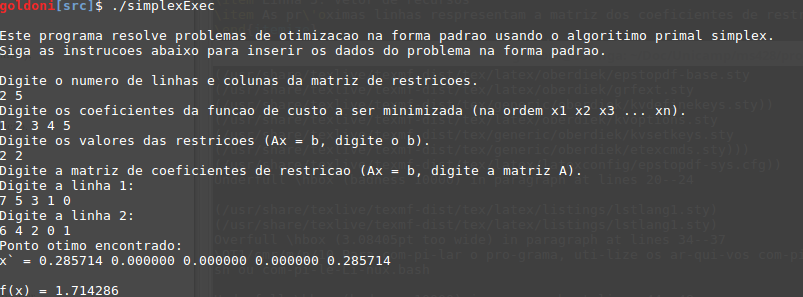
\includegraphics[width=0.95\textwidth]{simplexEntradas.png}
\end{figure}
\\
Como sa\'ida, o programa retorna:
\begin{itemize}
\item Caso encontre a solu\c{c}\~ao, o programa retorna o ponto encontrado e o valor da fun\c{c}\~ao,
\item Caso o problema n\~ao encontre solu\c{c}\~ao fact\'ivel, o programa retorna a seguinte frase: "Problema infactivel!!! Ainda existem variaveis artificiais diferentes de zero na solucao encontrada com BigM"
\\
\item Caso o problema tenha infin\'itas solu\c{c}\~oes, o programa retorna a seguinte frase: "Problema nao tem solucao finita!!"
\end{itemize}
%--------------------------------------------------------------------------------------------------
\section{Discus\~ao}
\section{Conclus\~ao}
\end{document} 
